\chapter{Crowdsourcing strategies in Pl@ntNet citizen based learning platform}
\label{chap:plantnet}
\enlargethispage{3\baselineskip}

\begin{keypointstwomargins}{Pl@ntNet}{-2cm}{-1cm}
        \textbf{Key points -- Crowdsourcing plant species}
        \begin{enumerate}[leftmargin=*]
        \item Aiding botanists in plant species identification is a challenging task. Species are often visually close and their identification requires expert knowledge.
        \item Pl@ntNet is a citizen science platform that allows users to upload images of plants and receive a list of possible species.
        \item The collaborative aspect of Pl@ntNet allows users to vote on the species they think are present in the image and contribute to new labeled data, which is then used to train a computer vision and help new identifications.
        \end{enumerate}

        \textbf{Contributions -- Exploration of Pl@ntNet label aggregation strategy}
        \begin{enumerate}[leftmargin=*,start=4]
        \item We release and evaluate the current Pl@ntNet label aggregation and compare it to other strategies.
        \item We release a subset of Pl@ntNet with images url and collected labels in the South Western European Flora of more than $6$ million observations and $800$ thousand users in a large-scale classification setting.
        \item We discuss how to integrate the current model's predictions in the votes aggregation. This is a challenging task due to the iterative aspect of Pl@ntNet: the current data helps train the next generation of models iteratively.
        \end{enumerate}
\end{keypointstwomargins}

While crowdsourcing is advertised to collect a large number of data easily, with strategies to mitigate the noise, openly available datasets are still scarce and with a low number of classes ($K\leq 10$ in general).
In this chapter, we focus on the Pl@ntNet platform, a citizen science platform for plant species recognition.
One of the challenges in this classification setting is the large number of possible species ($K>10^4$).
After presenting the platform and voting system, we will investigate the current label aggregation strategy in Pl@ntNet.
We compare it with other strategies that can handle this large number of classes, workers and tasks.
Finally, we propose to improve the current algorithm by taking advantage of the Pl@ntNet pipeline.

Note that in previous chapters, the crowdsourcing experiments concerned workers paid to answer multiple tasks.
In Pl@ntNet, contributions are by volunteers and the tasks are not paid.
We thus slightly adapt the vocabulary used in this chapter to reflect this difference.
People voting are called users.
The tasks are observations of plants (detailed in \Cref{sub:obs_plantnet_what}) for which we wish to identify the species.
To reflect this change, we write $\mathcal{U}$ the set of all users. Each user $u$ has a unique identifier used as an index, and we denote $\mathcal{U}_i$ the set of users that have voted on observation $i$.
We thus have $\mathcal{U} = \bigcup_{i\in [n_\texttt{task}]} \mathcal{U}_i$.
The vote of user $u$ on observation $i$ is denoted $y_i^u\in [K]$.


\section{Crowdsourcing for plant species identification}
\label{sec:introducing_plantnet}

Computer vision models are a great aid in plant species recognition in the field \citep{vidal2021perspectives,borowiec2022}.
However, to train them we need large annotated datasets.
These datasets are often created thanks to citizen science approaches, collecting both reliable and useful information \citep{brown2019potential}.
Among existing plant recognition applications, the Pl@ntNet citizen science platform \citep{affouard2017pl} enables global data collection by allowing users to upload and annotate plant observations.

We first introduce the problem of labeling a plant observation and the complexity of plant taxonomy. Then, we present the Pl@ntNet platform and its voting interface.
Finally, we discuss the current label aggregation strategy and propose ways to improve it.

\subsection{Plant taxonomy generalities}
First, we need to understand the complexity of plant taxonomy.
Our goal here is to briefly present the taxonomy of plants.
Plants are divided following a hierarchy, from the most general to the most specific ranks of taxa: kingdom, division, class, order, family, genus, and species according to the International Code of Nomenclature for algae, fungi and plants (ICN) \citep{turland2018international}.
Each of these units of biological classification is called a taxon (taxa in plural).
Further secondary ranks also exist (tribe, subspecies, variety, form) but we will focus on the main ones.

Roughly, an example of taxonomy levels is:
\begin{itemize}
        \item Kingdom: separates plants from animals, fungi, and bacteria -- \emph{e.g} Plantae.
        \item Division: separates spore (\emph{angiosperms}) or seed (\emph{gymnosperms}) reproduction with specific characteristics. There are 14 plant divisions in total.
        \item Class: Angiosperms are divided into Monocotyledons(grasses, yuccas, etc.) and Dicotyledons (angiosperms with pair of leaves).
        \item Order: Group of families with common characteristics -- \emph{e.g} \emph{Cucurbitales} (generally ends with \emph{-ales}).
        \item Family: Plants with similar flower, fruit and seed structures -- \emph{e.g} \emph{Begonaias and Allies}.
        \item Genus (genera in plural): First part of the plant's scientific name (capitalized and italicized) -- \emph{e.g} \emph{Begonia}.
        \item Species: a group of organisms capable of producing fertile offspring -- \emph{e.g} \emph{Begonia ferox}. If the species is unknown it is called \emph{sp.} or \emph{spp.} for plural.
\end{itemize}

In the case a plant is a hybrid -- a cross between two species -- it is written with an x as in \emph{Begonia} x \emph{semperflorens}. The position of the x indicates if it is the hybridization between two genera or species.
For example, the × \emph{Agroelymus hajastanica} is the hybridization of the \emph{Agropyron cristatum} and the \emph{Elymus repens} -- note that the genera are aggregating into a resulting genus.
Similarly to the x, a + is used to indicate a transplant chimera between two plants.
For example, the + \emph{Laburnocytisus adamii} results of the transplant of two individuals with different genera: the \emph{Laburnum anagyroides} and the \emph{Cytisus purpureus}.


\subsubsection{Checklists and referentials}

The plant name is generally composed of only two parts: the genus and the species.
In this work, we do not consider vernacular names -- the common names of plants -- as they can vary from one region to another.
Botanists have created checklists of accepted plant species.

One of the largest is the International Plant Names Index (IPNI) \citep{IPNI2024}.
The IPNI is a database of the published names and indicates which names are validly published.
It does not take into account the taxonomic status of the names -- the chronological changes and synonymity.
The World Checklist of Vascular Plants (WCVP) \citep{govaerts2021world} is an international collaborative database of taxa that provides the latest nomenclatural and taxonomic information on vascular plants -- \emph{clubmosses}, \emph{horsetails}, \emph{ferns}, \emph{gymnosperms} (including conifers), and \emph{angiosperms} (flowering plants).
The data from WCVP is the backbone for Plants Of the World Online (POWO) \footnote{\url{https://powo.science.kew.org}} which is an interface to access more information on individual species as their distribution for example.

There are multiple other checklists and databases such as The Plant List (TPL) \citep{PlantList2013}, the Catalogue of Life (CoL) \citep{cachuela2006towards}, Leipzig Catalogue of Vascular Plants (LCVP) \citep{freiberg2020leipzig} \emph{etc.} For a more exhaustive comparison of these databases we refer the reader to \citet{schellenberger2023big}.
The Global Biodiversity Information Facility (GBIF) \citep{telenius2011biodiversity} is an openly accessible network of shared knowledge about biodiversity on Earth.
They currently regroup $105$ different sources of taxonomy\footnote{\url{https://www.gbif.org/fr/dataset/d7dddbf4-2cf0-4f39-9b2a-bb099caae36c}}.

These checklists are the backbone of any botanical project as they provide a reference for the species names, their taxonomic status, and synonymic contributions.
Synonyms are not rare in plant taxonomy and can be due to different reasons such as the same species being described by different botanists, at different times, in different regions of the world.
As an example, in WCVP there are $357347$ plant species and $565200$ synonyms for those species.

Moreover, note that checklists might not always cover all the species and synonyms from one another.
For example, the \emph{Pilosella officinarum} Vaill. is listed in POWO with $161$ possible synonyms  -- $141$ accepted synonyms and $20$ illegitimate -- while in the GBIF it is listed with $241$ possible synonyms.
In the Pl@ntNet database, synonyms are only considered at the species level, resulting in $22$ possible accepted synonyms for this species.

\begin{figure}[tbh]
        \centering
        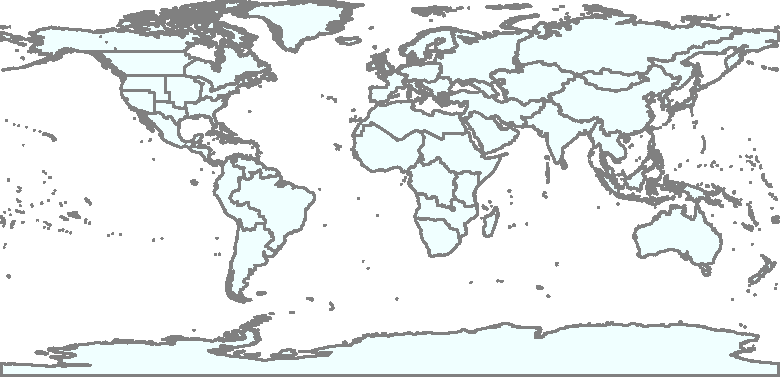
\includegraphics[width=.95\textwidth]{./images_plantnet/level2.pdf}
        \caption{Regional areas at level 2: subcontinental botanical regions of the world.  }
        \label{fig:level2}
\end{figure}

The international system groups areas of the world at different levels to record plant distributions and have standardized comparisons. This system is called the World Geographical Scheme for Recording Plant Distributions (WGSRPD) \citep{brummitt2001world}. The first level represents the nine botanical continents -- Europe, Africa, Asia-Temperate, Asia-Tropica, Australasia, Pacific, Northern America, Southern America and Antarctic.
The second level is the subcontinental regions of the world -- see \Cref{fig:level2} for a representation. It divides each botanical continent between $2$ and $10$ subdivisions. For example, Europe is divided into Northern, Middle, Southwestern, Southeastern and Eastern Europe.
Levels 3 and 4 include states, provinces or botanical areas.
In Pl@ntNet, level 2 is used to filter the species that can be observed in a given area and adapt the models' predictions.
In addition, users can specify to which flora -- either a level 2 subdivision or a Pl@ntNet project like "Useful plants" or "World Flora" -- they wish to associate their contribution.

\subsection{What is a plant observation?}
\label{sub:obs_plantnet_what}

\begin{figure}[bth]
        \centering
        \begin{minipage}[b]{0.3\textwidth}
            \centering
            \includegraphics[width=\textwidth,height=4cm]{./images_plantnet/quadra1.JPG}
        %     \caption{Caption for Image 1}
        %     \label{fig:image1}
        \end{minipage}
        \hfill
        \begin{minipage}[b]{0.3\textwidth}
            \centering
            \includegraphics[width=\textwidth,height=4cm]{/images_plantnet/quadra2.jpeg}
        %     \caption{Caption for Image 2}
        %     \label{fig:image2}
        \end{minipage}
        \hfill
        \begin{minipage}[b]{0.3\textwidth}
            \centering
            \includegraphics[width=\textwidth,height=4cm]{./images_plantnet/quadra3.jpeg}
        %     \caption{Caption for Image 3}
        %     \label{fig:image3}
        \end{minipage}
        \caption{Quadrats used in the field to estimate the abundance of species. They are often in a hard rectangle shape material like wood or soft with meters of ribbon to delimit the surface. (\textcopyright Pierre Bonnet)}
        \label{fig:quadrats}
    \end{figure}

Contrary to classical datasets, Pl@ntNet observations are not a single image but a set of images taken by a user in the field.
A single image of a plant might not be enough to identify the species.
More images of different parts of the plant -- leaves, flowers, fruits, \emph{etc.} -- are needed to correctly identify the species and mimic a botanist's behavior while it is surely not the same and we can not replace such expertise.

In the field, some recommendations include\footnote{\url{https://ibis.geog.ubc.ca/biodiversity/eflora/identification.html}} but are not limited to:
\begin{itemize}
        \item the type of plant: a shrub, an herb, a fern, \emph{etc.}
        \item physical traits of the plant -- height, color range, hairy (length, width), texture (velvety, rough, smooth), is it stingy, thorny? \emph{etc.}
        \item position and number of leaves, flowers (symmetrical, shape), fruits or seeds (size, flesh), \emph{etc.}
        \item blooming period
        \item the type of bark -- smooth, rough, flaky, color, color changes depending on the season
        \item the roots -- if safely available for both the identifier and the identified plant -- to see rooted stems, rhizomes, bulbs or tubers. A horizontal expansion of the roots can be a sign of a rhizome.
        \item the aroma (minty, pungent)
        \item grown habits -- bushy, sprawling around, erected, vine-like
        \item other species around, abundance of the species
        \item \dots
\end{itemize}

Once these criteria are gathered, the botanist can identify possible species.
To filter out the possible species, the botanist will also consider the habitat -- sand, marshes, rocky fields -- the elevation -- sea level, mountain -- and the region to narrow the confusion.
The use of a determination key can also help the identification.

\begin{figure}[bth]
        \centering
        \begin{minipage}[b]{0.49\textwidth}
            \centering
            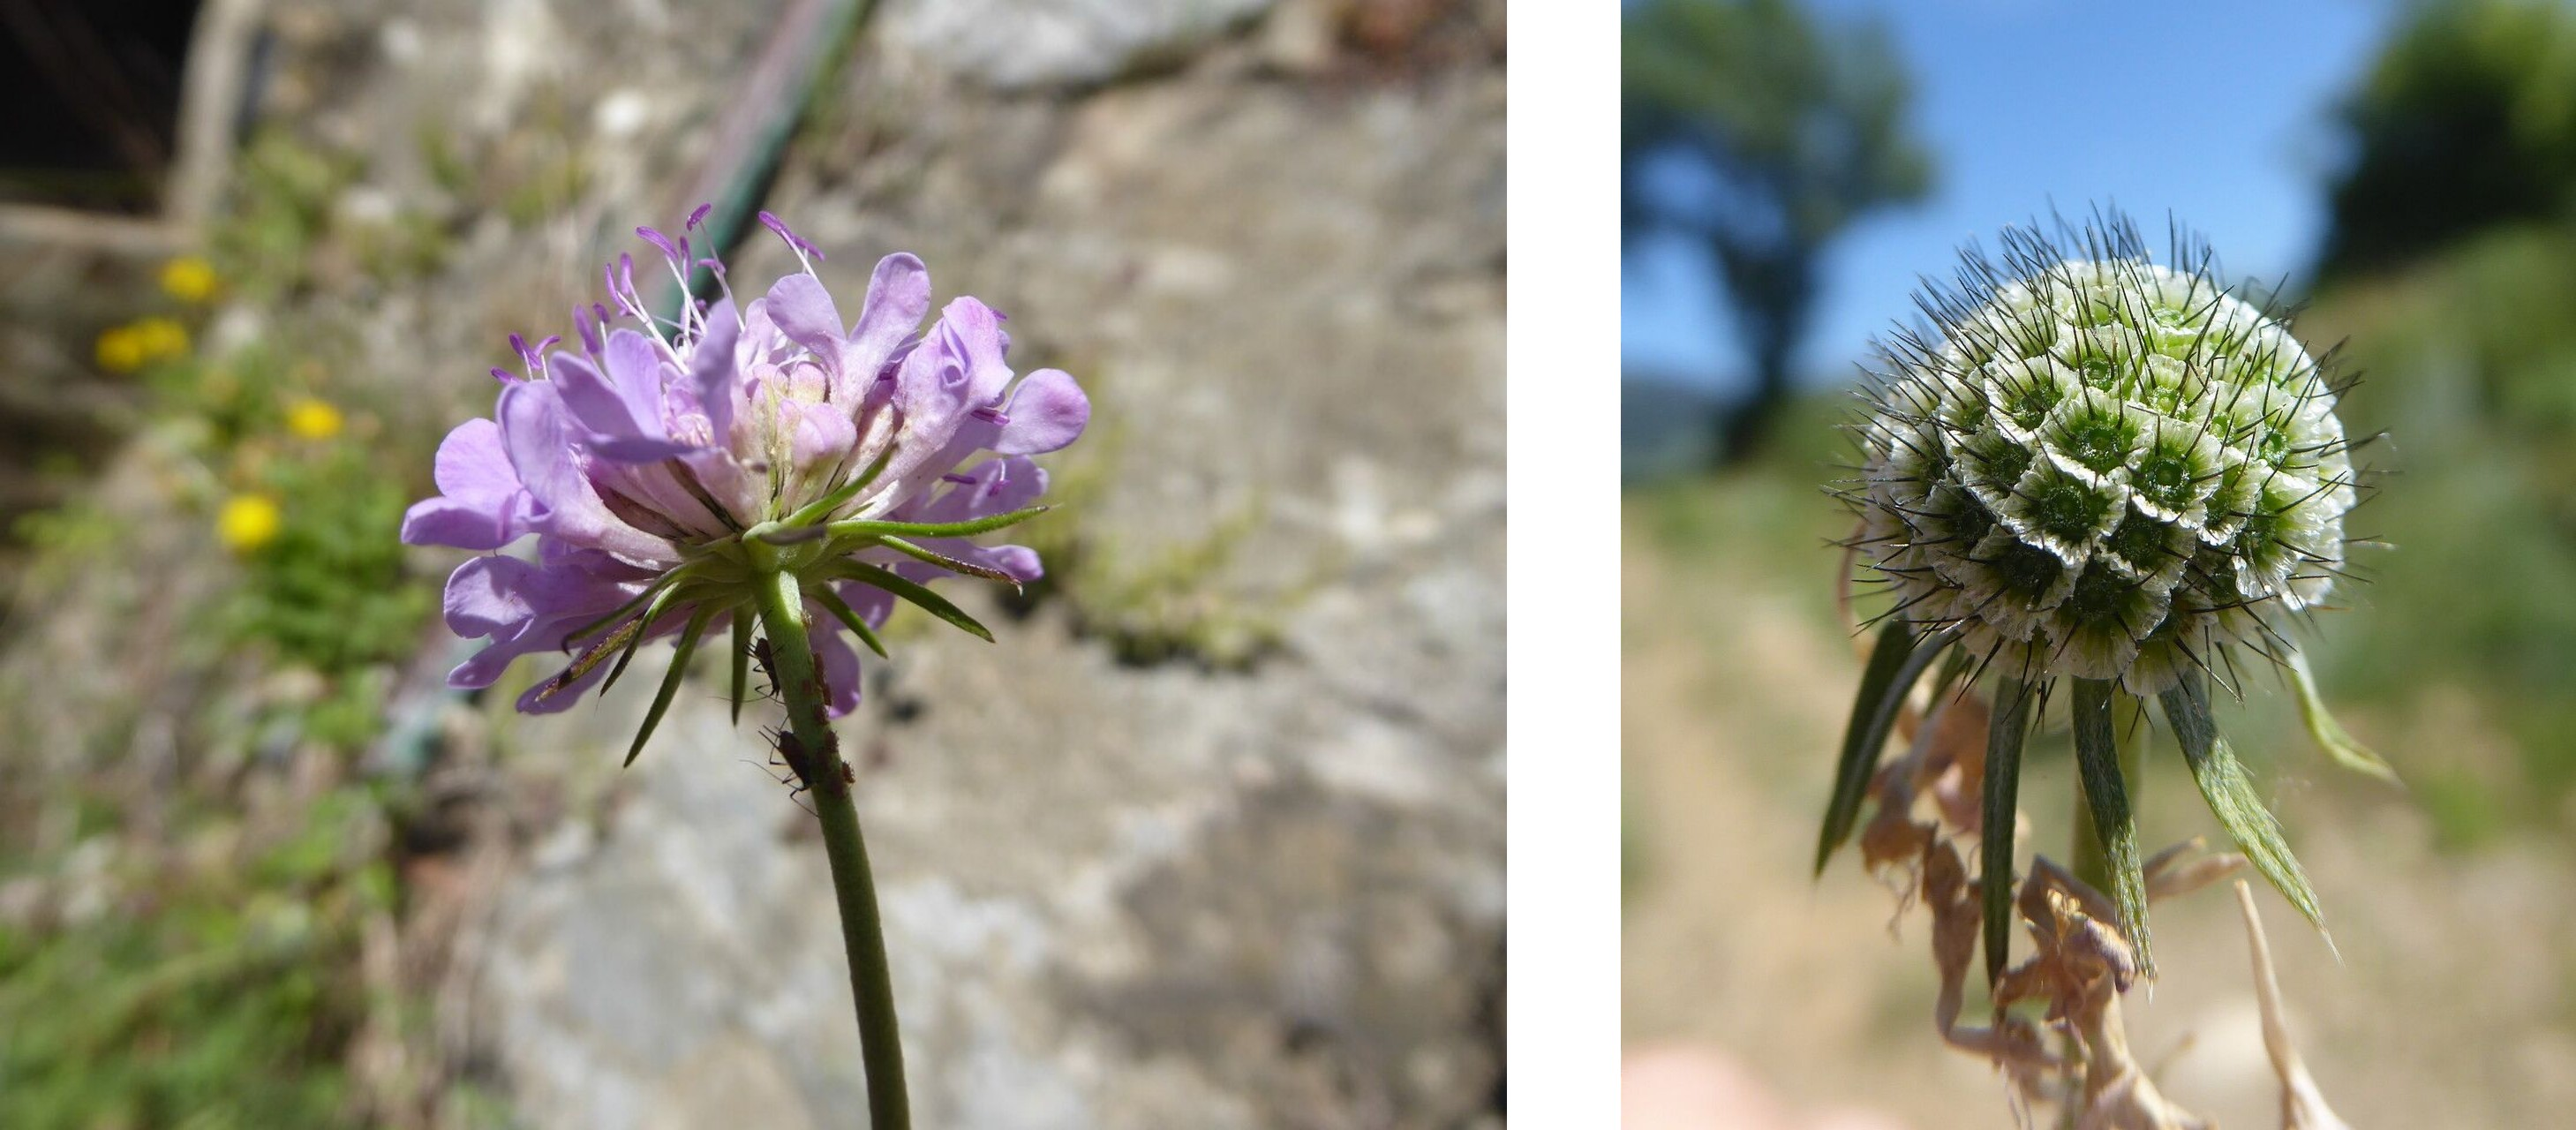
\includegraphics[width=\textwidth,height=4cm]{./images_plantnet/scabiosa.jpg}
            \caption*{Observation of a \emph{Scabiosa columbaria} L. (\textcopyright Llandrich anna)}
        %     \label{fig:image1}
        \end{minipage}
        \hfill
        \begin{minipage}[b]{0.49\textwidth}
            \centering
            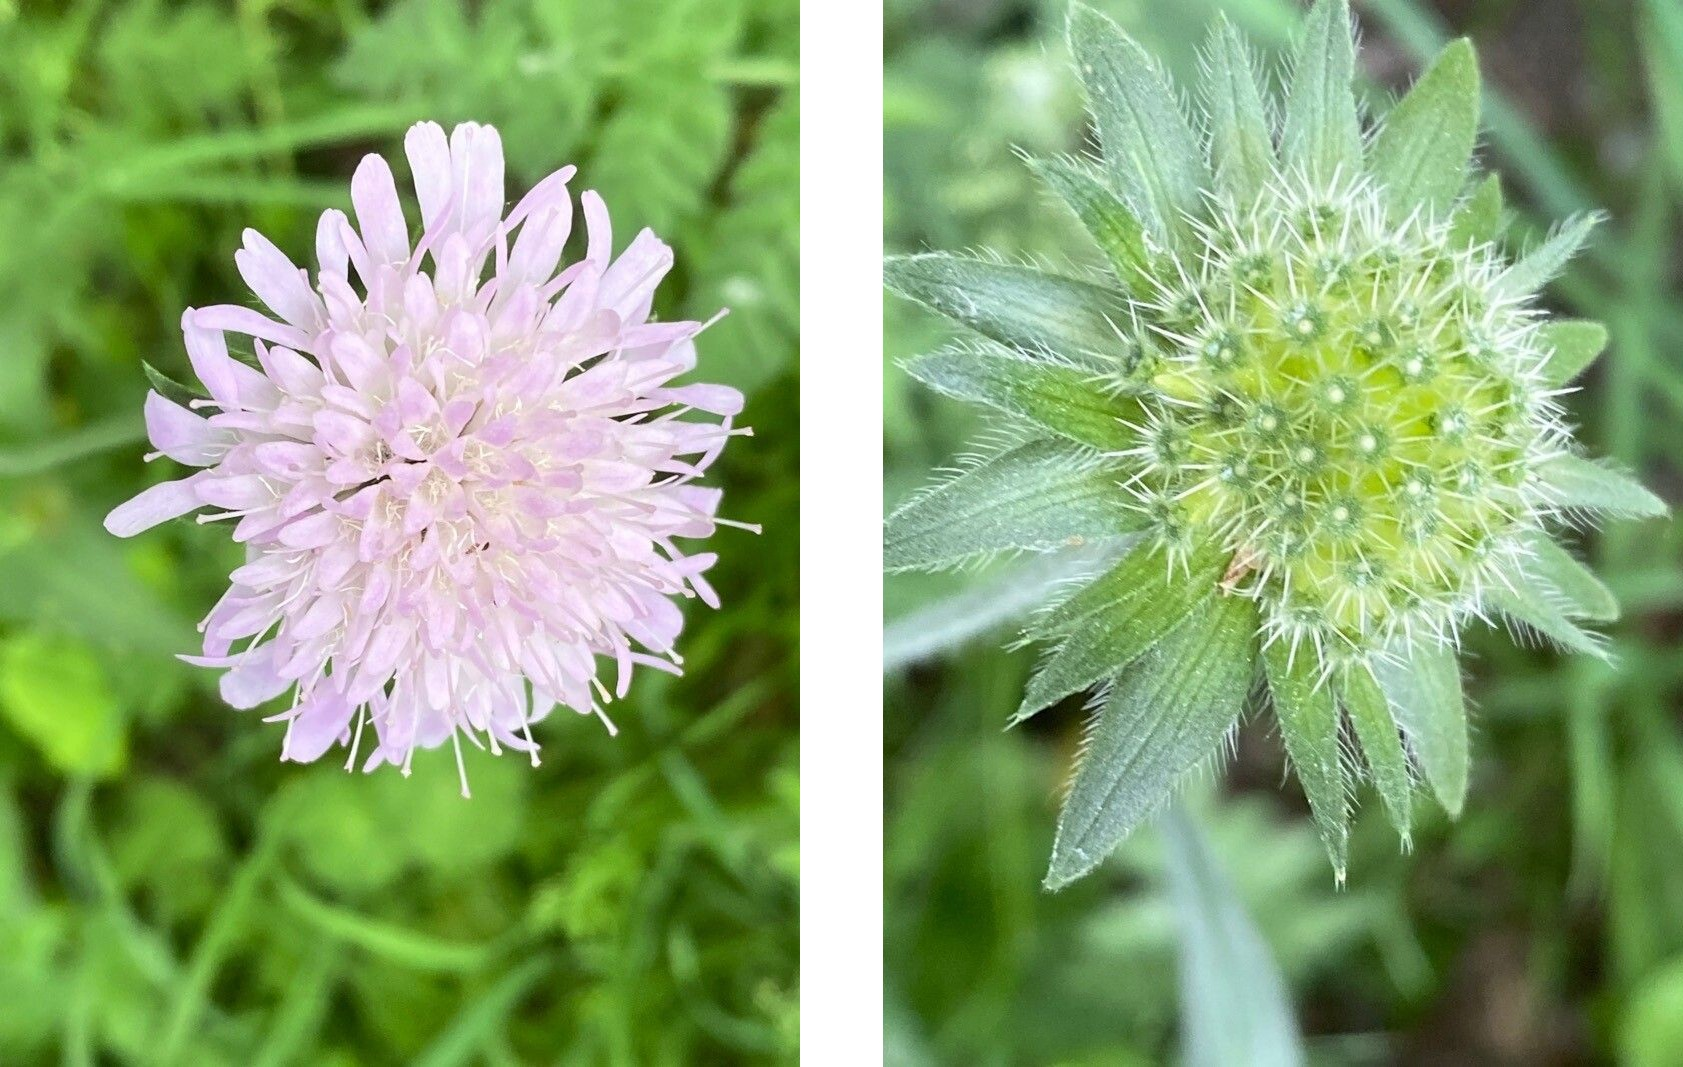
\includegraphics[width=\textwidth,height=4cm]{./images_plantnet/knautia.jpg}
            \caption*{Observation of a \emph{Knautia arvensis} (L.) Coult. (\textcopyright Francois Mansour)}
        %     \label{fig:image3}
        \end{minipage}
        \caption{Two observations of different species known to be difficult to identify from one another: a \emph{Scabiosa columbaria} L. and a \emph{Knautia arvensis} (L.) Coult. The flowers are visually close, but the leaves from the bottom view on the \emph{Scabiosa} and the structural differences in the second photo allow a clear identification.}
        \label{fig:scabiosa-knautia}
    \end{figure}

In practice, botanists use quadrats -- plots of ground of a specific size -- to count the number of species in a given area and estimate the abundance of each species. Such quadrats are shown in \Cref{fig:quadrats}.


Most of these criteria (like the aroma, texture or habitat), can be difficult or even impossible yet to be gathered from multiple images, and much less from a single one.
Hence, the use of multiple images is crucial to correctly identify the species or at least narrow down the possible species.
Botanists will observe multiple organs (flower, fruit, leaf), from different angles (a flower from the bottom view can have specific traits not visible from the side).
These characteristics can be transmitted via multiple images for the same observation.
We give an example in \Cref{fig:scabiosa-knautia} of two species that are visually close but can be distinguished using multiple images in the same observation.

\subsection{Presenting the voting interface}

\subsubsection{Author contribution.}

\begin{figure}[H]
        \centering
        \begin{minipage}[b]{0.38\textwidth}
            \centering
            \includegraphics[width=\textwidth]{./images_plantnet/pothos_marble.png}
            \caption*{Observation of a plant which necessitates identification (\textcopyright Tanguy Lefort). The image is sent to Pl@ntNet's computer vision model for identification. A similarity search is performed to present similar pictures for each proposed species.}
        %     \label{fig:image1}
        \end{minipage}
        \hfill
        \begin{minipage}[b]{0.55\textwidth}
            \centering
            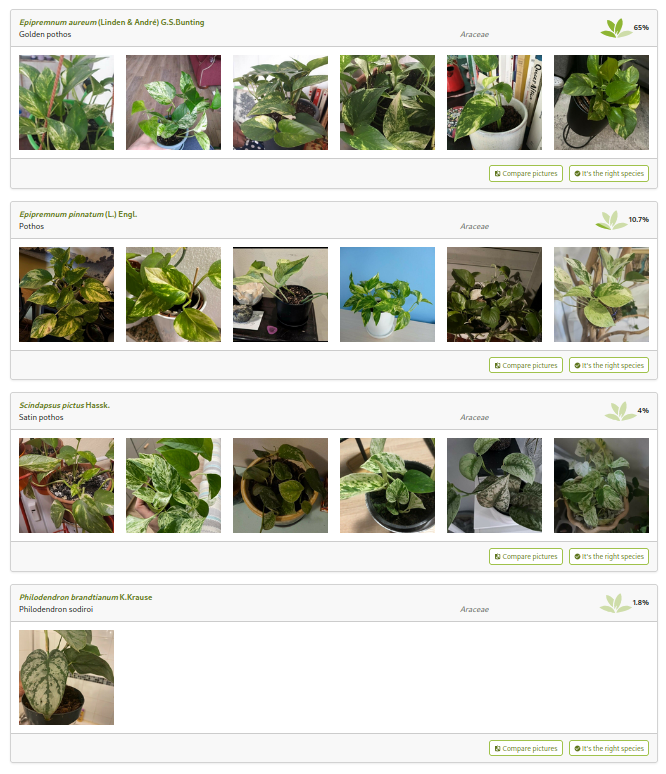
\includegraphics[width=\textwidth]{./images_plantnet/pothos_marble_plantnet.png}
            \caption*{Pl@ntNet identification results}
        %     \label{fig:image3}
        \end{minipage}
        \caption{From an image query, Pl@ntNet outputs possible species. For visual aid, close-looking images are also shown for each proposed species. The user can then click on the \emph{compare picture} button to make their choice. Then, the user can vote on the species by clicking on \emph{It's the right species} button. Here the probability of \emph{Epipremnum aureum} (Linden \& André) G.S.Bunting to be the right species is $65\%$ -- also known as \emph{Pothos aureus} Linden \& André.}
        \label{fig:pothos_id}
\end{figure}

In Pl@ntNet, an observation is a set of images taken by a user in the field.
The author user can then upload these images to the platform.
The platform will then propose a list of possible species for the observation with the associated predicted probabilities and other images that are close-looking to the picture taken.
The author can then vote on the species they think are present in the observation as illustrated in \Cref{fig:pothos_id}.

The vote is guided by the computer vision model predictions (see \Cref{sub:pipeline_plantnet}) and other pictures selected via a similarity search algorithm.
This similarity search is important as the same species can have different visual presentations at multiple stages of its life cycle.
The similarity search is based on the features from the last layer of Pl@ntNet's network.
These features are hashed using the Random Maximum Margin Hashing algorithm \citep{joly2011random} and then an approximate $k$-nearest neighbors is applied \citep{joly2008posteriori}.

If a user disagrees with the model's predictions, they can enter the name of the species freely in the input box as shown in \Cref{fig:pothos_sharing}.
The user input is guided by the name of possible species in the currently selected flora.

% \begin{wrapfigure}[14]{l}{.55\textwidth}
        \begin{figure}[tbh]
        \centering
        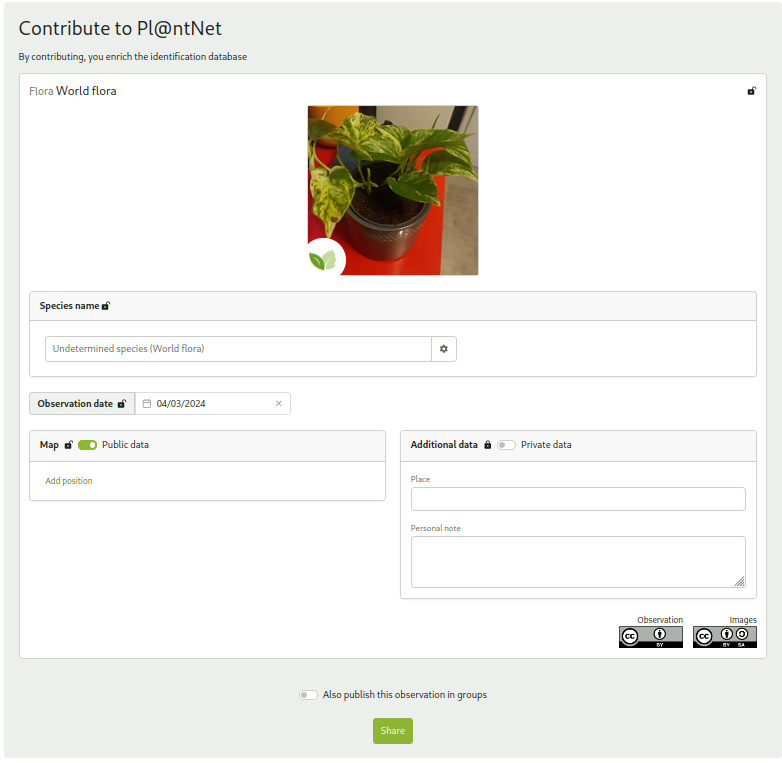
\includegraphics[width=.65\textwidth]{./images_plantnet/free_sharing_pothos.png}
        \caption{The author can select one of the model's predicted species or input freely the name of a species. The user input is guided by the name of possible species in the currently selected flora (here World Flora). Note that by clicking on the gear icon, a user can change the flora.}
        \label{fig:pothos_sharing}
        \end{figure}
% \end{wrapfigure}

The author can also input any text freely -- hence adding possible noisy votes.
At this stage, there is no filter performed on the existence of the given species in the database.
The author can also share the location of the observation, and add additional inputs in a specific reserved field -- the habitat, the aroma or any other feature they would like to share.
Some users unfortunately might mistake the different fields and input information as the species name, a cleaning step is thus a necessary step in the platform.

\subsubsection{Other users contributions.}

Once the observation is shared online, it is time for others to enter the collaborative playground.
Any user can visit the \emph{identify} Pl@ntNet platform and vote on observations.
The view is as presented in \Cref{fig:others_plantnet}.

\begin{figure}[tbh]
        \centering
        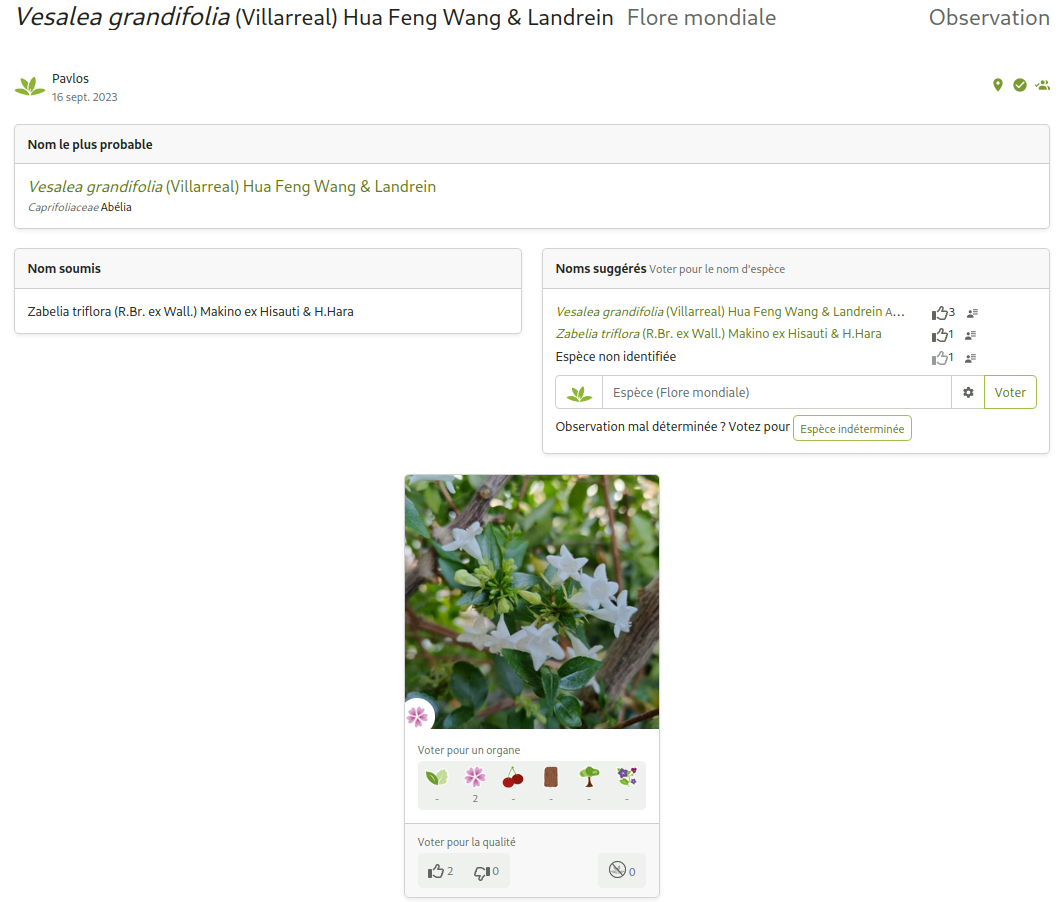
\includegraphics[width=.95\textwidth]{./images_plantnet/plantnet_others.png}
        \caption{View of observations as a user (\textcopyright Pavlos). The current prediction is shown, with the initial species proposed. Suggestions from other users are on the right, with a field to propose your thoughts or accept someone else's. Anyone can vote for the organ shown in the image -- in this case, users agree on the flower. The quality is accepted by 2 users and there is no vote to reject the observation based on the fact there is no plant in the actual image.}
        \label{fig:others_plantnet}
\end{figure}

The initial author determination -- if existing -- is shown, with the current prediction.
In the \emph{suggested name} box, all registered species votes are shown with the number of agreements.
In \Cref{fig:others_plantnet}, 5 different users voted: 3 for the species \emph{Vesalea grandifolia} Villarreal Hua Feng Wang \& Landrein, 1 for the \emph{Zabelia triflora} (R.Br. ex Wall.) Makino ex Hisauti \& H.Hara and one user voted for \emph{undertermined} -- meaning they could not identify the species or there is not enough information provided to their knowledge to identify the species.
There is a field for a new vote, where the user is guided to propose an existing species but can enter any text freely.
By clicking on the Pl@ntNet icon next to it, the model's predictions are shown with the associated probabilities and close-looking examples to guide the identification as in \Cref{fig:pothos_id}.

In addition to the species, users (as authors) can vote on the organ shown in the image(s).
The organs can be a leaf, flower, fruit, bark, habit (form in which the plant grows) or other.
Users can approve or disapprove the quality of the image -- if the plant is not correctly visible, the image is blurry, or the organ is not visible.
If there is no plant in the image, they can also flag it with the \emph{no plant} button.

In the upper-right section of the presented observation, the user can see if the observation was associated with any geolocalisation, if the observation is considered as \textbf{valid} by the Pl@ntNet algorithm and if it was reviewed by others.
The \emph{valid} status is given by the Pl@ntNet algorithm presented in \Cref{sub:algo_plantnet} and is a proxy for the quality of the observation.

The iNaturalist platform uses a research grade status to indicate the quality of the observation\footnote{\url{https://www.inaturalist.org/posts/39072-research-grade}}:
\begin{itemize}
        \item there is a picture or recording of sound,
        \item the genus and/or species name of the organism are specified,
        \item the GPS coordinates are associated,
        \item the observation is timed and dated,
        \item the observatory is identified,
        \item there is at least a $2/3$ agreement consensus by users on the identified species.
\end{itemize}
In Pl@ntNet, the data quality is monitored by this \textbf{valid} status that depends on the estimated reliability of a user and the agreement of the community on the observation.
We explain in more detail the algorithm used to estimate the reliability of a user in \Cref{sub:algo_plantnet}.

\subsubsection{What is not an observation.}

Until now, we described what is an observation.
So, let us show examples of what isn't an observation.

\begin{figure}[bth]
        \centering
        \begin{minipage}[t]{0.25\textwidth}
            \centering
            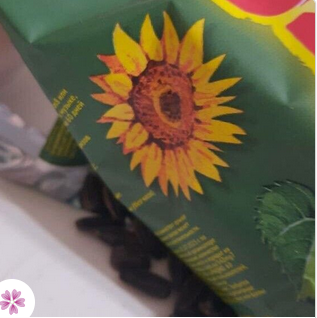
\includegraphics[width=\textwidth,height=4cm]{./images_plantnet/katyykkk_no_plant.png}
            \caption*{A drawing is not a plant (\textcopyright Katyykk)}
        %     \label{fig:image1}
        \end{minipage}
        \hfill
        \begin{minipage}[t]{0.25\textwidth}
            \centering
            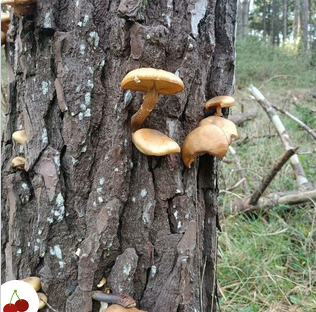
\includegraphics[width=\textwidth,height=4cm]{./images_plantnet/eugenio_perez_perez_shroom.png}
            \caption*{A fungus is not in the Plantae kingdom (\textcopyright eugenio perez perez)}
        %     \label{fig:image3}
        \end{minipage}
        \hfill
         \begin{minipage}[t]{0.47\textwidth}
                \centering
                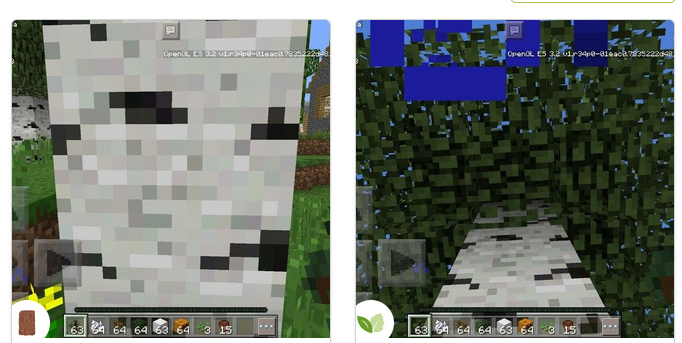
\includegraphics[width=\textwidth,height=4cm]{./images_plantnet/PA0L0_D1_B3LL0_minecraft.png}
                \caption*{A video game tree (minecraft version of a birch tree) is not a real plant. (\textcopyright PA0L0\_D1\_B3LL0)}
            %     \label{fig:image3}
            \end{minipage}
        \caption{Three examples of images that are not plant observations.}
        \label{fig:not_an_observation}
    \end{figure}

More generally, drawings -- even realistic -- of plants or photos of images of plants are not considered plant observations.
The same goes for fungi, which are not part of the Plantae kingdom and thus are not identified by Pl@ntNet.
Finally, images of video games -- even if they represent plants -- are not considered plant observations.
We show examples of these in \Cref{fig:not_an_observation}.
Photos of people, animals, pornographic images or any other object that is not a plant are also not considered plant observations.
These images are flagged, removed from the platform and are not used to train the models.

Another possible issue is the presence of multiple species in the same observation.
These observations are flagged as \emph{malformed}, we provide an example in \Cref{fig:malformed_observation}.
Users can cast their vote to indicate that the observation is malformed and should not be considered.

\begin{figure}[htbp]
        \centering
        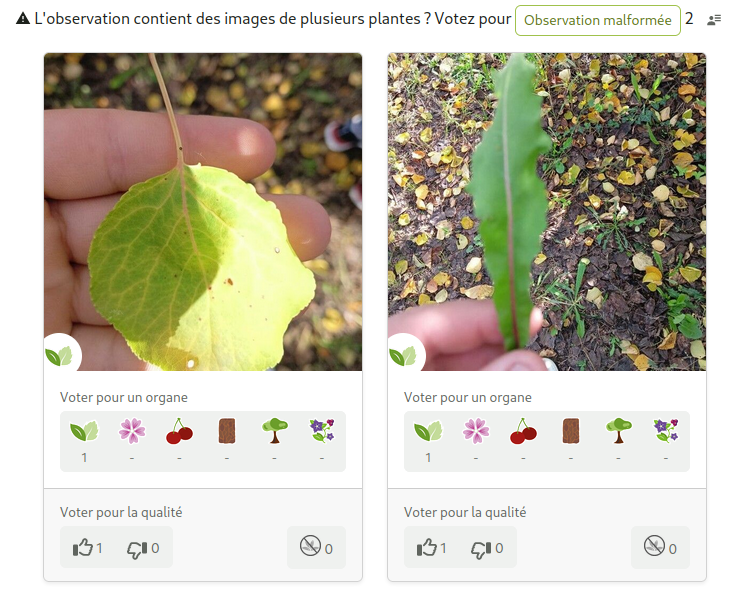
\includegraphics[width=.75\textwidth]{./images_plantnet/maformed_leonardo_liberati.png}
        \caption{Malformed observation: each image is associated with a different species (\textcopyright Leonardi Liberati).}
        \label{fig:malformed_observation}
\end{figure}

\subsection{A step in a bigger pipeline}
\label{sub:pipeline_plantnet}

\begin{figure}[thb]
        \centering
        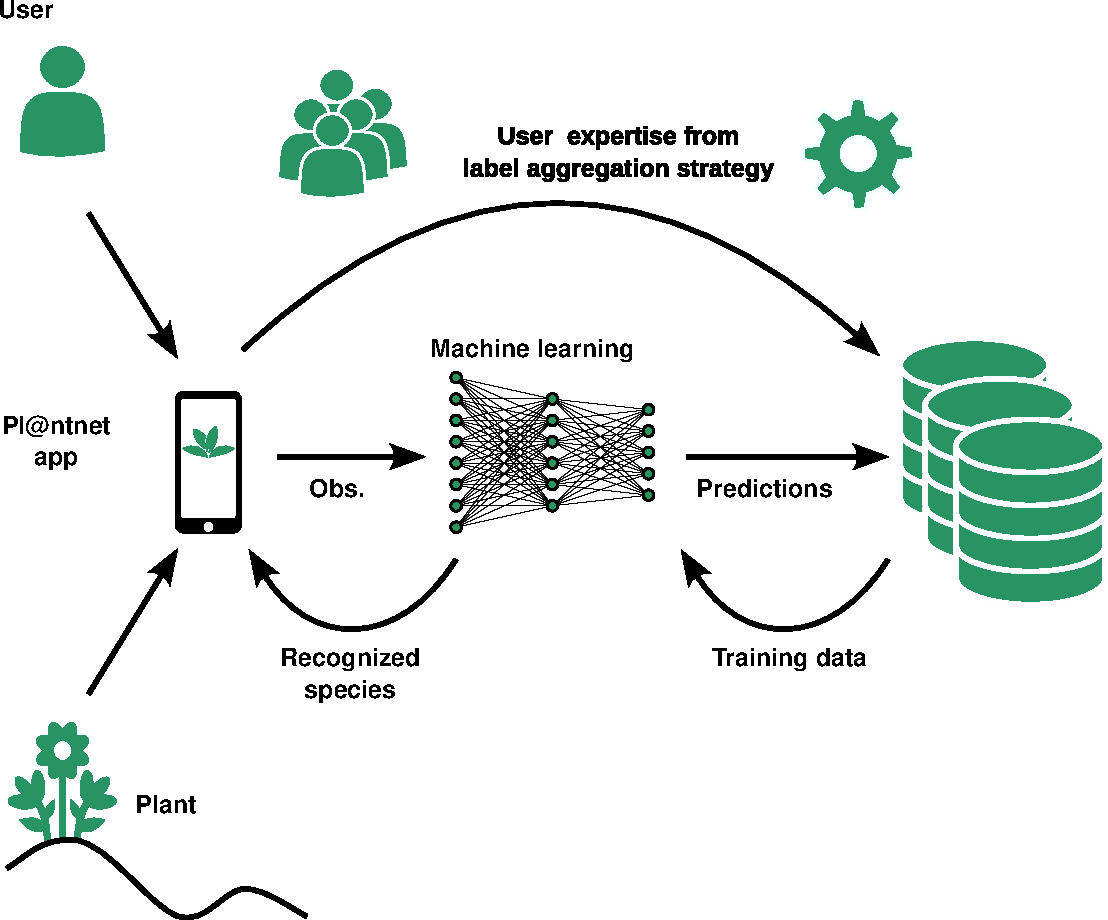
\includegraphics[width=.65\linewidth]{images/plantnet_schema_global_green.pdf}
        \caption{Pl@ntNet system of human-AI interaction for plant species recognition. Users take their plant observations in the Pl@ntNet application. A prediction is output by the AI model. Users can validate the prediction or propose another species. The whole votes collection is used to evaluate user expertise and actively revise observations identifications.}
        \label{fig:plantnet-system}
    \end{figure}

The gathering and aggregation of votes is only a part of the Pl@ntNet pipeline.
Schematized in \Cref{fig:plantnet-system}, the Pl@ntNet system is a loop between curating the data and training a computer vision model.
The label aggregation algorithm is presented in detail in \Cref{sec:aggregation_plantnet}.
Let us briefly address the computer vision model part.

At the time of writing, the model in use in Pl@ntNet is DINOv2 \citep{oquab2024dinov2} a transformer-based network.

XXX ask more details to JCf


\section{Pl@ntNet's label aggregation strategy}
\label{sec:aggregation_plantnet}

As we discussed in \Cref{sec:introducing_plantnet}, plant species identification is a task that requires skills to recognize morphological traits (shapes, measurements, environments and specific characteristics).
A large number of users with diverse skills have participated in gathering plant observations and helped improve the training dataset of our computer vision model.
Their participation is based on votes that they can cast on others' observations, or by the initial species determination of their observation.
The quality of each vote is then processed by the algorithm presented in \Cref{sub:algo_plantnet}.

At the time of writing, this participatory approach has resulted in the collection of over 20 million observations, belonging to almost $\numprint{46000}$ species, by more than 6 million users worldwide. In total, more than $25$ million of images are shared in these observations.

Other citizen science projects such as iNaturalist \citep{van2018inaturalist} or eBird \citep{sullivan2009ebird} use a similar approach to collect data, but differ in their label aggregation strategy.
The iNaturalist project, with more than $2.5$ million users, records the votes at different taxonomic levels.
The resulting label is the aggregation of at least two votes on a species-level identification (or coarser or finer taxonomic level).
A taxon requires at least a two-thirds agreements among identifiers and all users have the same weight in the decision-making.
Over time, a taxon can be further refined by the community, debated or revoked.
eBird handles taxon quality control by using a checklist in each region for observers.
Quality verifications on the checklist are performed and, combined with user knowledge -- number of species and checklist submitted, number of flagged observations, discussions among local experts -- the observation taxon is accepted.
The eBird project also showed that monitoring species accumulation from observers can help to sort their skills \citep{kelling2015}. While they consider the species accumulation by hours spent on each collected observation, we present a strategy that takes into account the entire history of observations of the observer.


\subsection{Presentation of the algorithm}
\label{sub:algo_plantnet}

\begin{algorithm}[tbh]
        \caption{Pl@ntNet iterative weighted majority vote}
        \label{alg:plantnet_algorithm}
        \textbf{Input}: Votes as $(u, y_i^u)_{i\in [n_{\mathrm{SWE}}],u\in [n_\text{user}]}$ for each observation $i$ and user $u$ answering the voted species $y_i^u$, accuracy threshold $\theta_{\text{acc}}$, confidence threshold $\theta_{\text{conf}}$, weight function $f$, initial weight $\gamma>0$ \\
        \textbf{Ouptput}: Estimated labels $\hat y_i$ and validity indicator $s_i$ for each observation $i$
        \begin{algorithmic}[1]
            \STATE $\text{Initialize } \hat y_i = \mathrm{MV}\left(\{y_i^u\}_u\right) \text{ for each observation } i \in [n_{\mathrm{SWE}}]$
            \STATE $\text{Initialize user weights as } w_u = \gamma \text{ for each user } u \in [n_\text{user}]$
            \WHILE{$\text{not converged}$}
                \FOR{each observation $i\in [n_{\mathrm{SWE}}]$}
                    \STATE Compute label confidence: $\mathrm{conf}_i(\hat y_i) = \sum_{u\in \mathcal{U}_i} w_u \mathds{1}(y_i^u=\hat y_i)$
                    \STATE Compute label accuracy: $\mathrm{acc}_i(\hat y_i) = \mathrm{conf}_i(\hat y_i) / \sum_{k\in [K]} \mathrm{conf}_i(k)$
                    \STATE Compute validity indicator: $s_i = \mathds{1}( \mathrm{acc}_i(\hat y_i) \geq \theta_{\text{acc}} \text{ and } \mathrm{conf}_i(\hat y_i) \geq \theta_{\text{conf}})$
                \ENDFOR
                \FOR{each user $u \in [n_\text{user}]$}
                    \STATE Compute the number of valid identified species for authoring observations: \[n_u^\text{author} = |\{y_i^u\in [K] \,|\, y_i^u=\hat y_i, s_i=1, \mathrm{Author}(i)=u\}|\]
                    \STATE Compute the number of identified species by voting on other's observations: \[n_u^\text{vote}=|\{y_i^u\in [K]\,|\, y_i^u=\hat y_i, \mathrm{Author}(i)\neq u\}|\]
                    \STATE Compute the rounding number of identified species per user: \[n_u = \mathrm{Round}\left(n_u^\text{author} + \frac{1}{10}n_u^\text{vote}\right)\]
                    \STATE Transform number of estimated species per user into trust score: $w_u = f(n_u)$
                    \ENDFOR
                \STATE Update estimated labels with a weighted majority vote $$ \forall i \in [n_{\mathrm{SWE}}],\ \hat y_i = \argmax_{k\in[K]} \sum_{u\in \mathcal{U}_i} w_u\mathds{1}(y_i^u=k)$$
            \ENDWHILE
        \end{algorithmic}
    \end{algorithm}

Pl@ntNet label aggregation strategy relies on estimating the number of correctly identified species for each user.
Similar to other strategies, we rely on an EM-based iterative procedure \citep{Dempster_Laird_Rubin77} to estimate consecutively the users' skills and each observation's species. The detailed iterative algorithm is provided in \Cref{alg:plantnet_algorithm}.

The label aggregation strategy generates a trust indicator ($s_i$) on the observation that can reveal whether an observation is valid or not.
Notice that in \Cref{alg:plantnet_algorithm} we value $10$ times more authored observations than voting on other's observations -- if a user proposes a new observation with a label (species name) it is more useful than proposing a label by clicking.
Indeed, being on the field leads to more information on the environment and a better determination of the species.
Finally, note that an identified species is exclusively identified as author -- part of $n_u^\text{author}$ in \Cref{alg:plantnet_algorithm}) -- or as click -- part of $n_u^\text{vote}$ -- to avoid redundant skills.
%species are unequivocally identified as authors ($n_u^\text{author}$ in \Cref{alg:plantnet_algorithm}) or as votes on other's observations ($n_u^\text{vote}$).
The final number of species identified by users is the aggregation of these two terms: $n_u = \mathrm{Round}\left(n_u^\text{author} + \frac{1}{10}n_u^\text{vote}\right)$.


\subsection{Introducing a subset of Pl@ntNet to evaluate the current strategy}

\section{Integrating model predictions in the aggregation}

\subsection{Possible strategies}

\subsection{Can we trust our current predicted probabilities?}

\section{Conclusion}